\documentclass{article}

% if you need to pass options to natbib, use, e.g.:
% \PassOptionsToPackage{numbers, compress}{natbib}
% before loading nips_2016
%
% to avoid loading the natbib package, add option nonatbib:
% \usepackage[nonatbib]{nips_2016}

\usepackage[final]{nips_2016}

% to compile a camera-ready version, add the [final] option, e.g.:
% \usepackage[final]{nips_2016}

\usepackage[utf8]{inputenc} % allow utf-8 input
\usepackage[T1]{fontenc}    % use 8-bit T1 fonts
\usepackage{hyperref}       % hyperlinks
\usepackage{url}            % simple URL typesetting
\usepackage{booktabs}       % professional-quality tables
\usepackage{amsfonts}       % blackboard math symbols
\usepackage{nicefrac}       % compact symbols for 1/2, etc.
\usepackage{microtype}      % microtypography

\usepackage{graphicx}
\usepackage{subcaption}
\usepackage{enumitem}
\usepackage{url}
\usepackage{amsmath}
\usepackage{listings}
\usepackage{booktabs, multirow, array, tabularx}

\lstset{
    basicstyle=\footnotesize,
    escapeinside={\%*}{*)},
    tabsize=2,
    language=python,
    numbers=left
}
% CleverRef Setup
\usepackage[capitalize,noabbrev]{cleveref}

\title{Parallel Sparse Convolution for Deep Learning}

% The \author macro works with any number of authors. There are two
% commands used to separate the names and addresses of multiple
% authors: \And and \AND.
%
% Using \And between authors leaves it to LaTeX to determine where to
% break the lines. Using \AND forces a line break at that point. So,
% if LaTeX puts 3 of 4 authors names on the first line, and the last
% on the second line, try using \AND instead of \And before the third
% author name.

\author{
  Ravi Teja Mullapudi 
  \And
  Prashanth Menon
}

\begin{document}
% \nipsfinalcopy is no longer used

\maketitle

\begin{abstract}
Performing inference on high-resolution video and image data using
state-of-the-art deep vision models is computationally demanding.  At the
heart of deep learning models for computer vision is the convolution
operation which is a 3d filtering operation on high-dimensional features.
Improving the performance of convolution layers continues to be a key aspect
of enabling computer vision research. There have been several efforts to
improve the efficiency by switching to different representation domain (FFT,
Winograd).  Though transformations into different domains enables performing
fewer expensive operations, they do not account for the possibility of only
needing to perform the convolution sparsely across the image (the domain
transformation significantly reduces the sparsity). Given the high
redundancy between video frames or the sparse signal generated by sensors
like LIDAR one can determine the sparse spatial locations to perform the
convolution. In this project, we demonstrate that a simple parallel and
locality-aware implementation of sparse convolution is indeed competitive
with highly-tuned vendor implementations of dense convolutions which operate
in a transformed domain.
\end{abstract}

\newcommand{\floor}[1]{\lfloor #1 \rfloor}
\newcommand{\ceil}[1]{\lceil #1 \rceil}

\section{Background and Related Work}
\label{sec:bg-rw}
\textbf{Convolution Layer} 
The filtering operation typically used in convolutional neural networks referred
to as the convolution layer is shown in Equation~\ref{eqn:conv}. The operation
takes as input features $I$, the filter coefficients $F$, and produces the
output features $O$.

\begin{equation}
O_{b, h, w, k} = \sum_{c=0}^{C}\sum_{y=0}^{F_h} \sum_{x=0}^{F_w} I_{b, S h+y, S
    w+x, z} * F_{k, c, y, x}
\label{eqn:conv}
\end{equation}

The features and the filter coefficients are represented as 4d tensors of the
following shapes:
\begin{align*}
& I:B \times H \times W \times C \\
& O:B \times (\ceil{(H - F_h + 2P)/S}) \times (\ceil{(W - F_w + 2P)/S}) \times K \\
& F:C \times K \times F_h \times F_w
\end{align*}
$B$ is the size of the batch of input features. $H$ and $W$ are the spatial
height and width of the input feature map. $S$ is the spatial stride at which
the filtering is performed on the input (sampling rate). $P$ is the amount of
padding added to the input to handle boundary conditions. $F_h$ and $F_w$ are
the spatial height and width of the filters. $C$ and $K$ are the input and
output feature dimensions respectively. The operation can be parallelized across
many dimensions and mapping the operation to modern hardware CPUs, GPUs, FPGAs
and other accelerators has been a topic of extensive
research~\cite{vasilache2014fast, lavin2016fast, liu2018efficient,
jia2018optimizing, tsai2016performance, truong2016latte, chetlur2014cudnn, chen2017eyeriss}. The main
challenge is efficient implementation is effectively utilizing the parallelism
offered by the architecture and while maintaining data locality.

\textbf{Spatial Sparsity} In settings where the input data is sparse or highly
redundant (consecutive frames of video) the convolution operation can only
performed in spatial locations where the input signal is present or changes
significantly. Figure~\ref{fig:frames} shows frames captured from one of the
onboard cameras in an autonomous driving car moving. Despite being captured a
low frame rate there is a significant region of the input that remains unchanged
at the pixel level. Feature representations in deeper layers of a network are
more robust to pixel-level changes and would exhibit even higher levels of
sparsity~\cite{shelhamer2016clockwork}. Recent work~\cite{ren2018sbnet} has show
the effectiveness of sparse block convolutions on sparse 3d LIDAR data.

\begin{figure}[h]
	\centering
\begin{subfigure}{0.3\textwidth}
	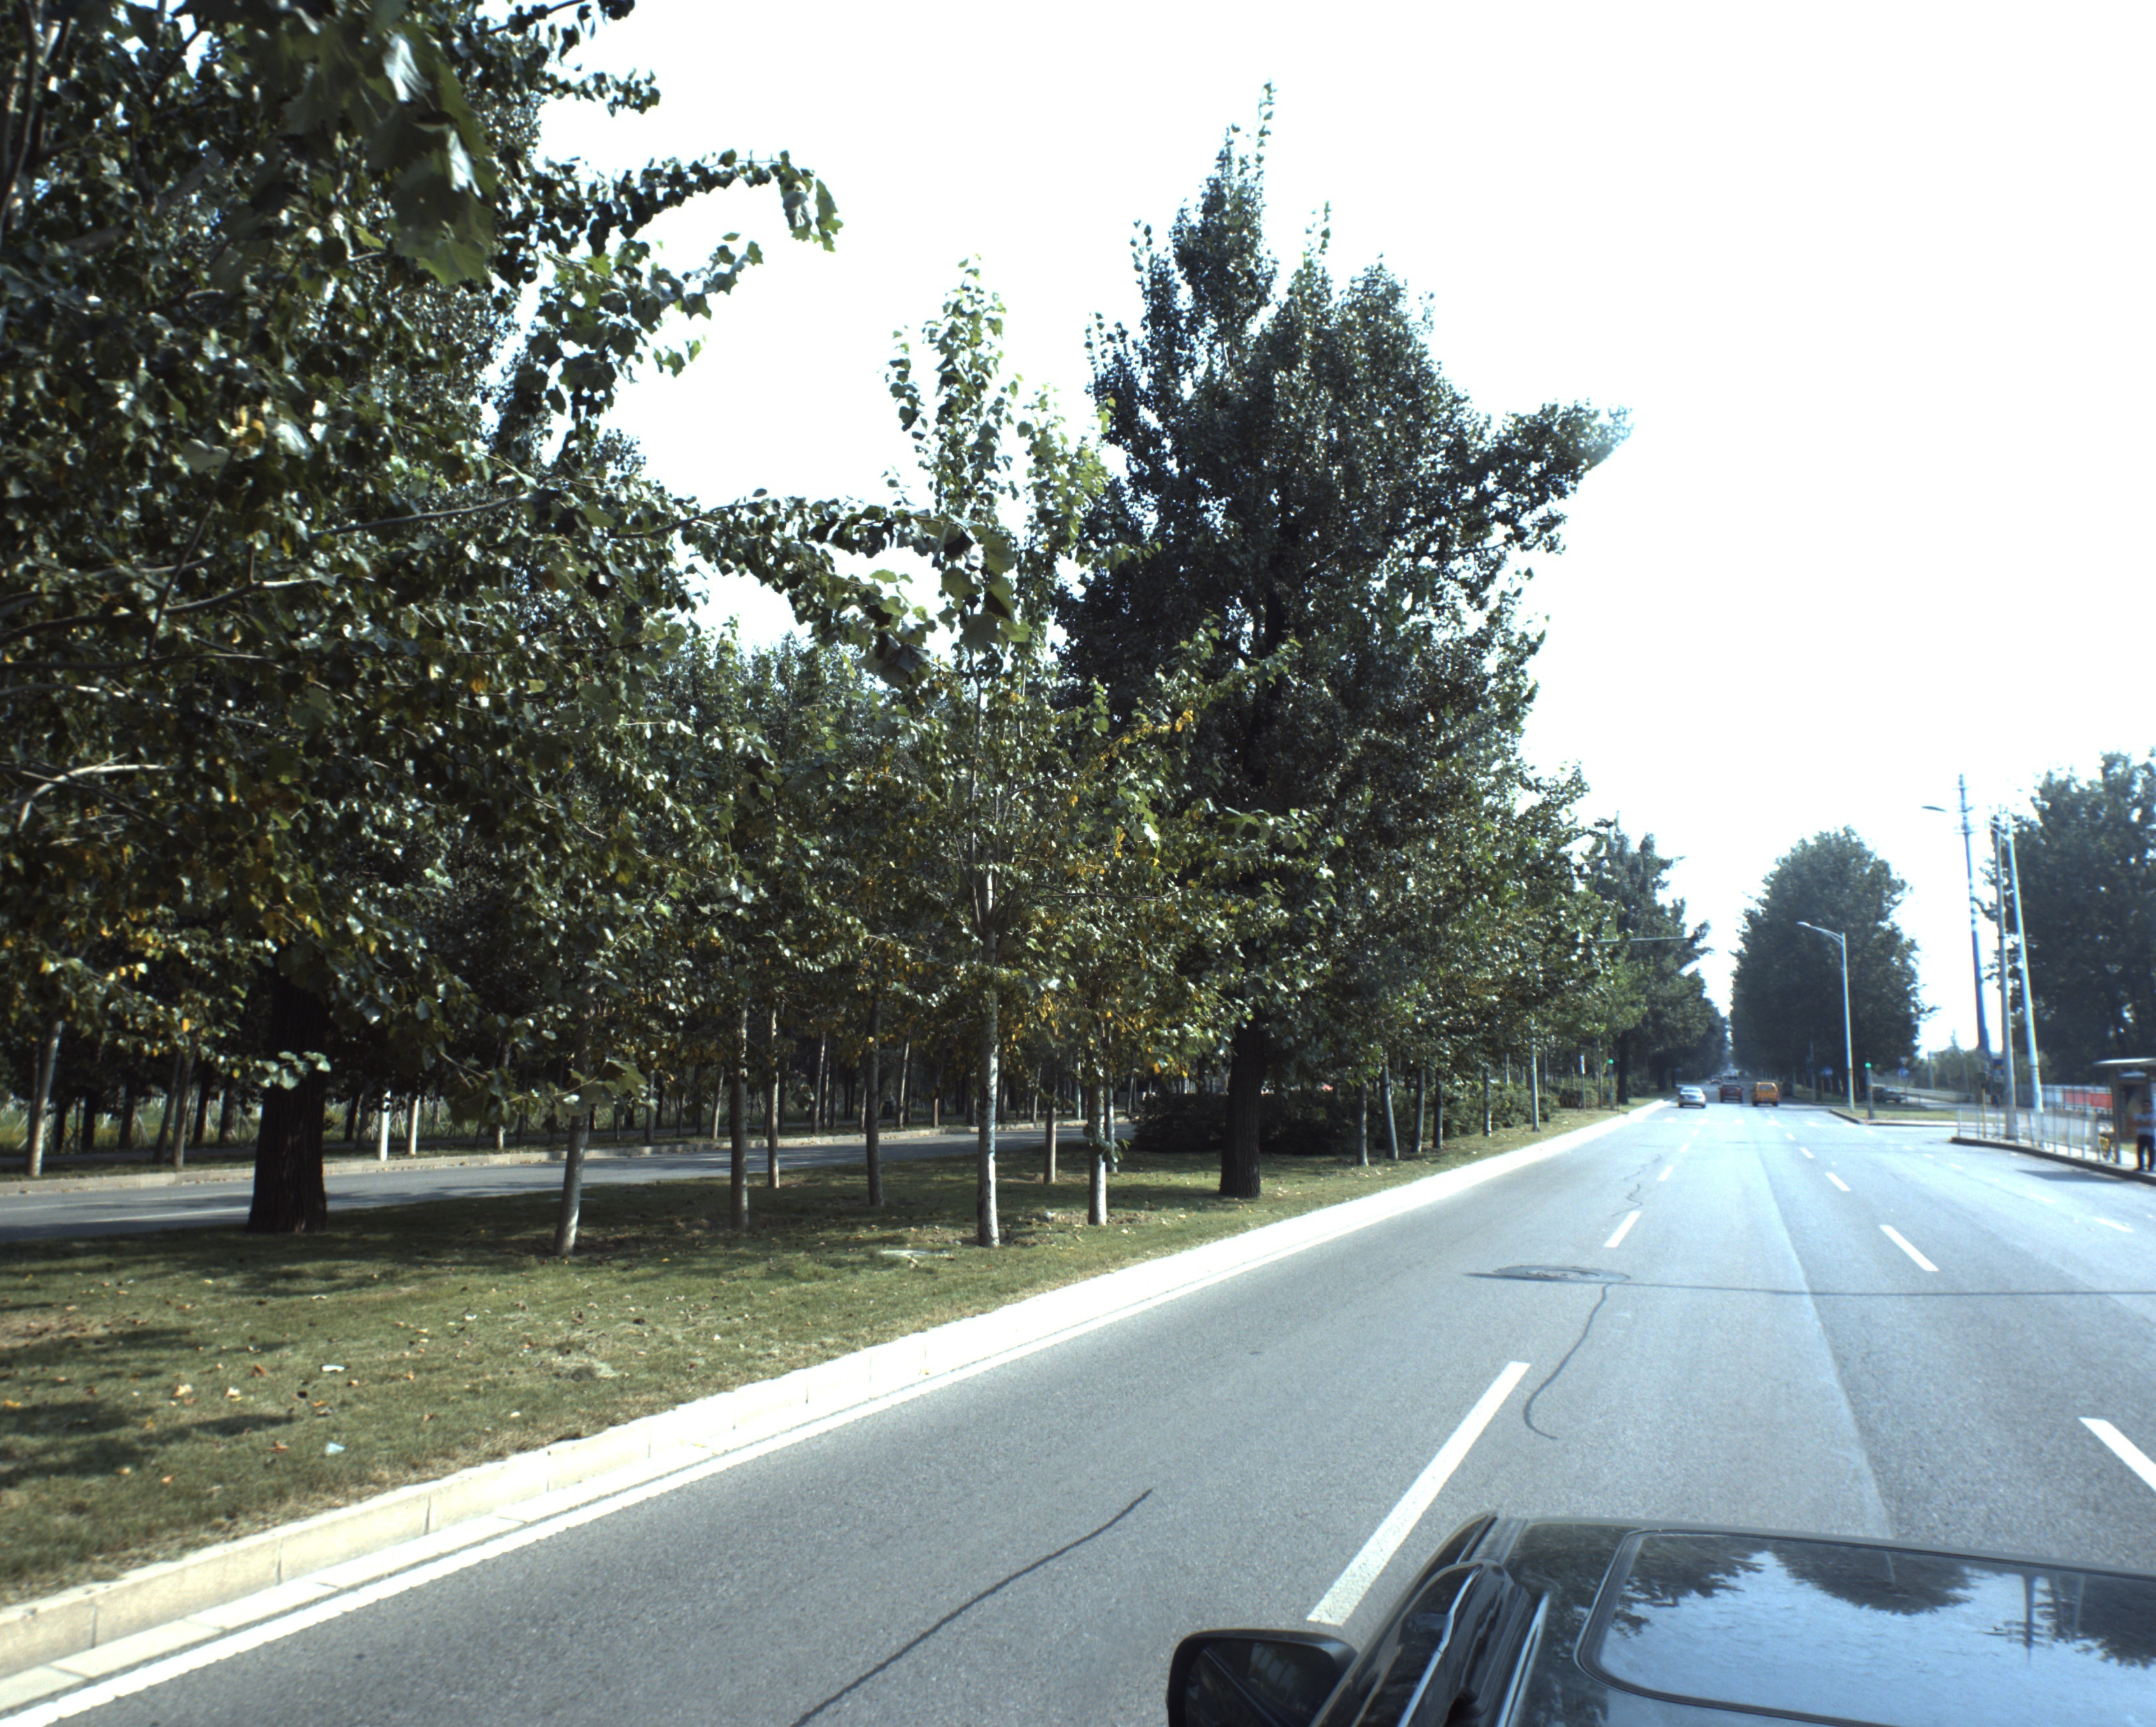
\includegraphics[width=\textwidth]{170908_061541883_Camera_5.jpg}
	\caption{Frame $n$}
\end{subfigure}
\hspace{0.1in}
\begin{subfigure}{0.3\textwidth}
	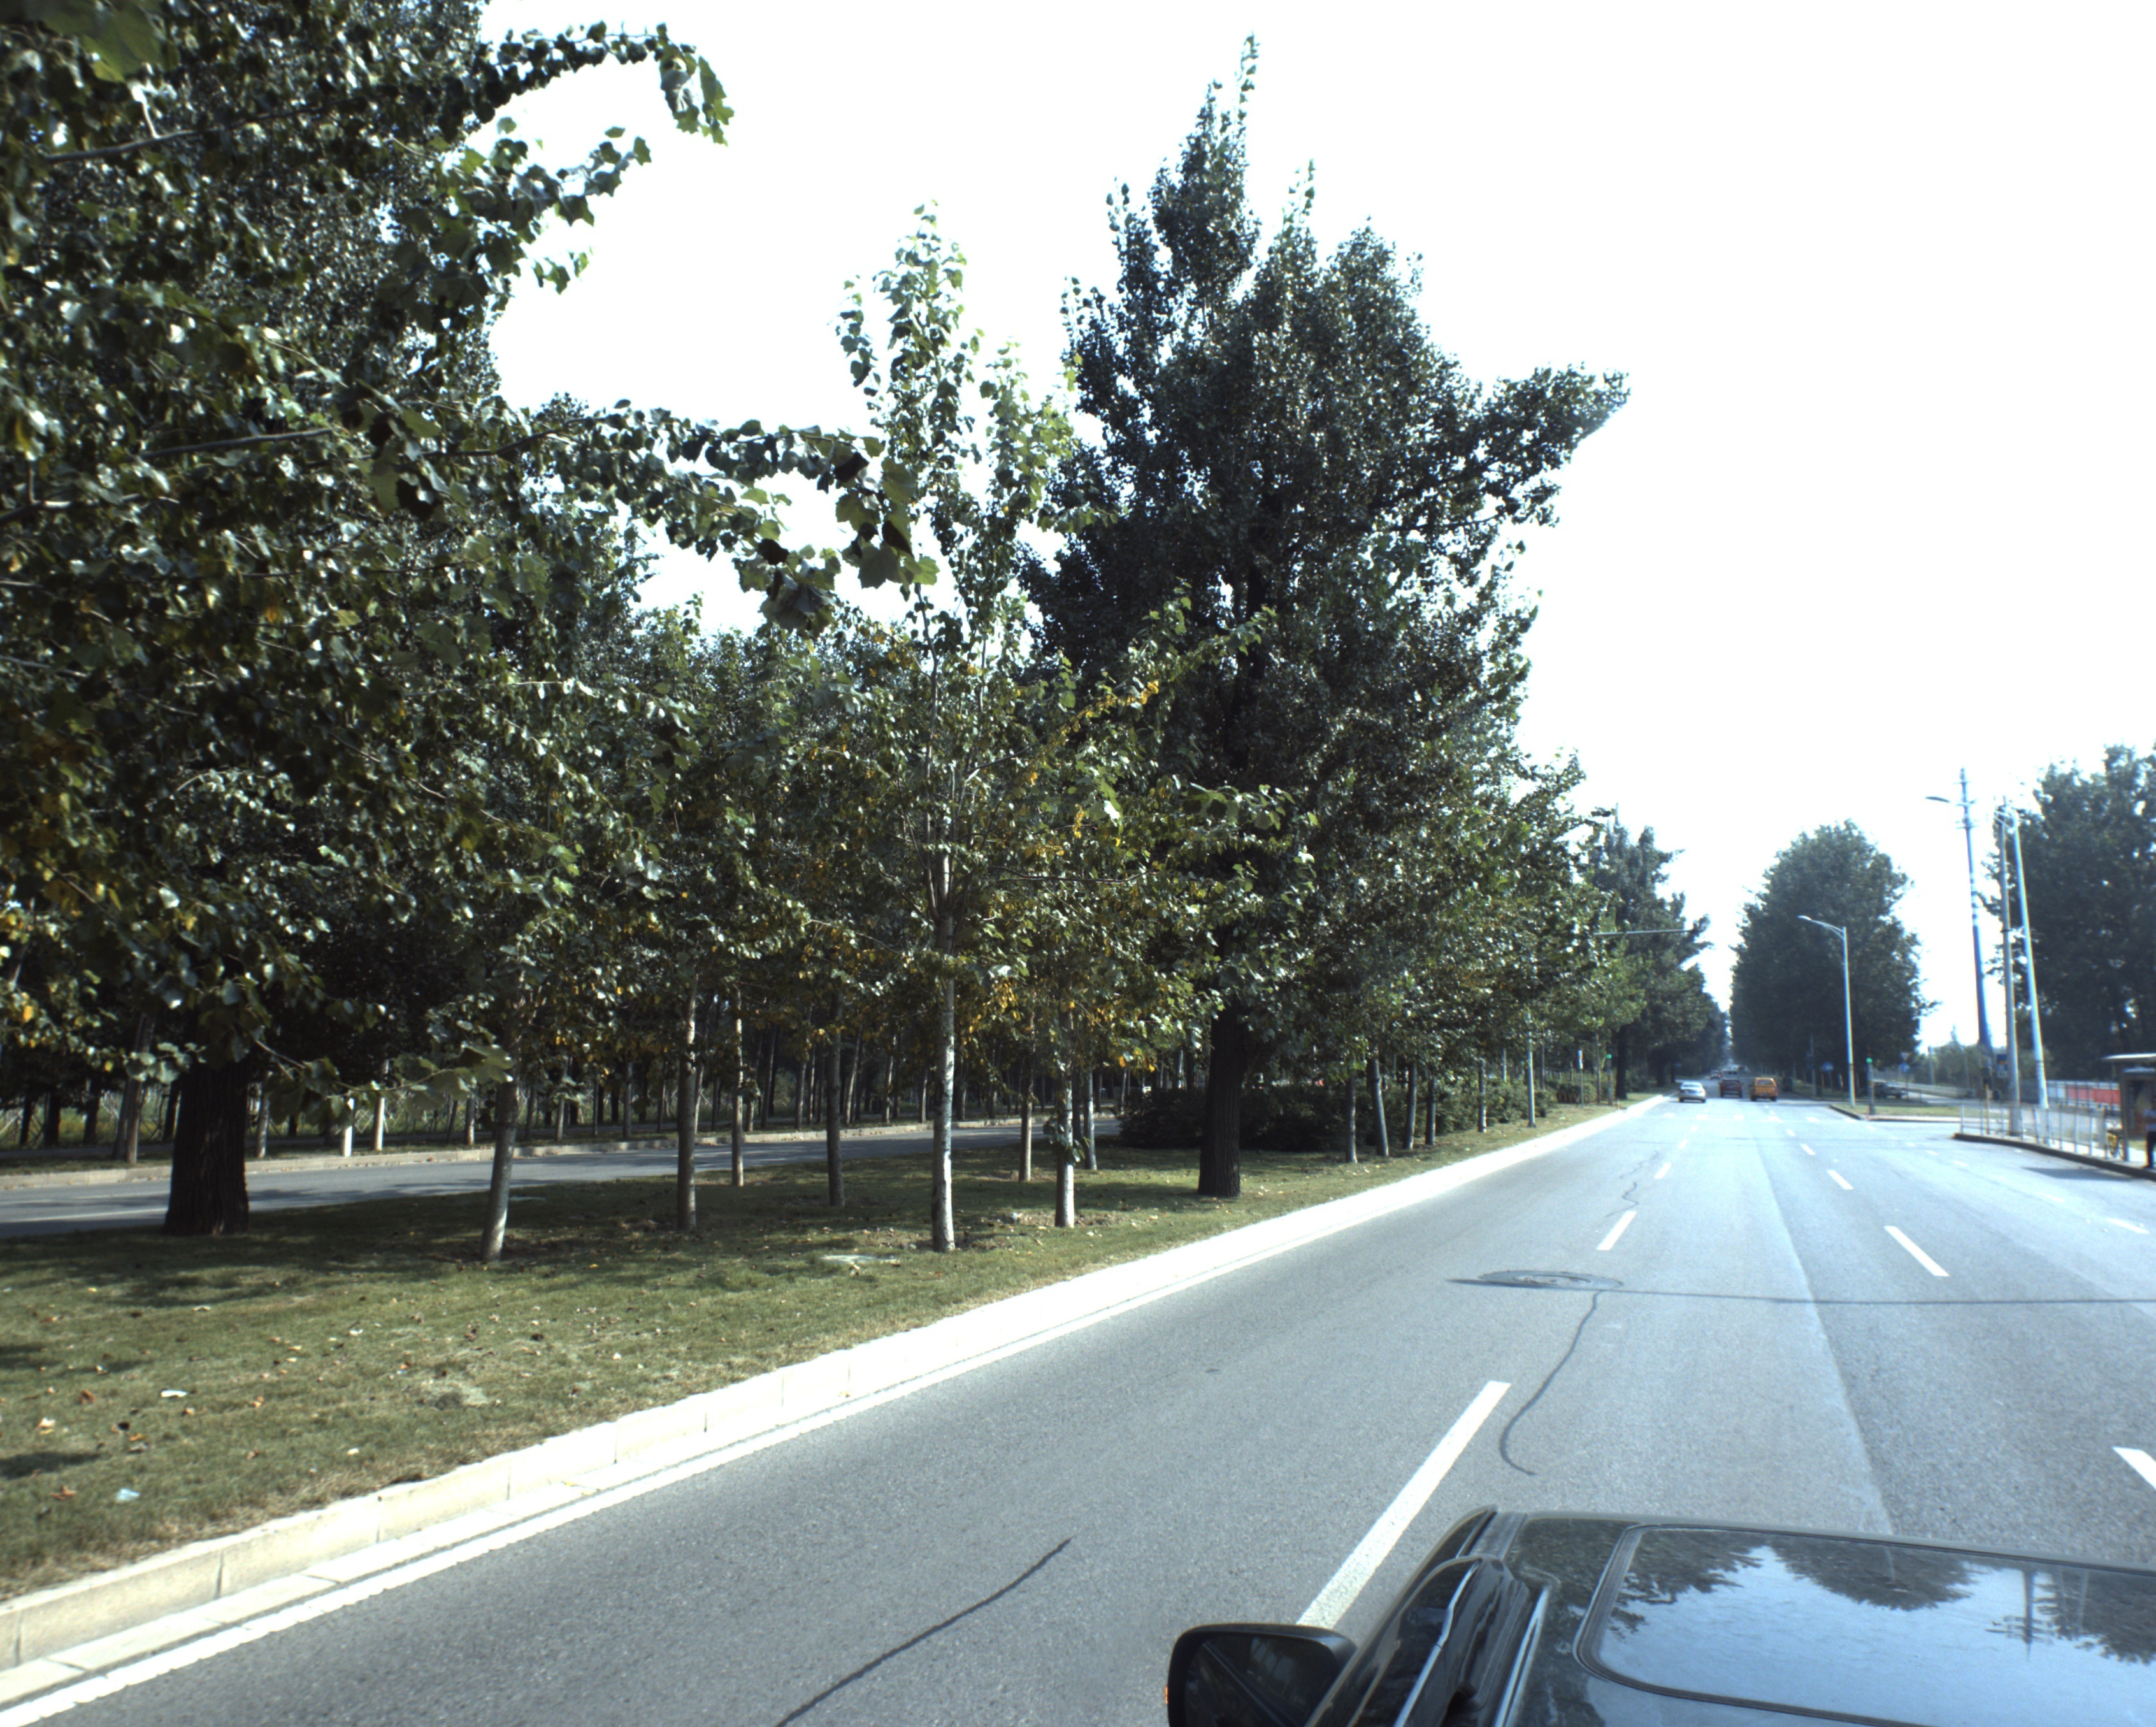
\includegraphics[width=\textwidth]{170908_061542022_Camera_5.jpg}
	\caption{Frame $n+1$}
\end{subfigure}
\begin{subfigure}{0.3\textwidth}
	
\includegraphics[width=\textwidth]{diff.jpg}
	\caption{Frame difference}
\end{subfigure}
\caption{Consecutive frames from a video stream and their difference at pixel
    level. The white region shows where the pixels have not changed.}
\label{fig:frames}
\end{figure}

\textbf{Direct vs. Indirect Convolution} Early implementation of the convolution
operation transformed the operation into a matrix multiply to leverage fast
vendor optimized linear algebra libraries for the target machine architecture.
Recent work~\cite{vasilache2014fast, lavin2016fast} has demonstrated that
performing the convolution in the other domains (FFT or winograd) yields
significant improvements in performance.  Indirect approaches involve
transforming the input features and the weights into a different domain,
followed by efficient operations in the transformed domain and an inverse
transformation back into the spatial domain. State-of-the-art models use filters
with small support ($3 \times 3$, $1 \times 1$), in this regime transformation
to the winograd domain is more effective than the FFT domain. Domain
transformation approaches do not work well with sparsity since spatial sparsity
cannot be effectively exploited during the
transformations~\cite{liu2018efficient}.  We demonstrate simple parallel and
locality-aware direct convolution performs comparably with highly tuned winograd
convolutions.

\section{Sparse Direct Convolution}
Our assumption is that the sparse spatial locations to compute the convolution
operation at is already determined. As we mentioned earlier this could be from
pixel or feature level differences in a video stream or from sparse input
signal. The locations are encoded by a mask $M$ which is a 3d tensor of shape $B
\times (\ceil{(H - F_h + 2P)/S}) \times (\ceil{(W - F_w + 2P)/S})$, $M_{b,h,w} =
1$ indicates that convolution needs to be performed at the location $h, w$ on
the $b^{th}$ input. Figure~\ref{fig:conv_algo} lists our parallel tiled
implementation of direct sparse convolution. The implementation is geared
towards a modern multi-core processor and convolution layers operate on inputs
with large spatial extent (which is common in semantic
segmentation~\cite{long2015fully} and object detection
models~\cite{he2017mask}). 

Our algorithm performs the operation in tiles which are done in parallel across
multiple cores. We use OpenMP to parallelize the tiles across the cores. The
tile sizes are chosen to ensure there is enough parallel work to keep the cores
saturated as well as to avoid imbalance due to the sparsity i.e., some tiles may
have more work than the others. Moreover, we use the OpenMP dynamic scheduler to
distribute the work across the cores to ensure workload balance. Line 6 shows
the parallel directive which performs all the iterations of loops on Lines 7-9
in parallel. By constraining the tile sizes in the spatial as well as the filter
output filter dimension the data locality is improved since there is data reuse
when the working set fits in the CPU caches.  This is similar to the blocked
matrix-multiply algorithm which improves data reuse.  Parallelizing across
the batch dimension is straightforward and not the main focus. Additionally, in
most inference settings there is a single input that needs to be processed fast
and our evaluation will focus on the single input per batch ($B=1$) setting.

Modern multi-core processors support parallelism at two levels one at the core
level and the other at the level of functional units (ALUs) which perform basic
operations like addition and multiplication. Typically there is support for
executing a single instructions on multiple data items called SIMD/vector
processing.  Current architectures have instructions which can perform either 8
or 16 floating point operations at the same time. One of the key challenges of
getting good performance on a modern processor is in effectively utilizing the
vector processing. Utilizing the SIMD units either requires the programmer to
explicitly use vector intrinsics or rely on compiler auto-vectorization. Our
initial experiments and analysis with gcc compiler showed that vector units were
not being utilized. OpenMP 4.0 added new directives which let the programmer
guide the compiler in generating good vector code. However, the new OpenMP
directives are only supported by the intel compiler which we use in our
evaluation. Lines 15-16 instruct the compiler to map the iterations of the loop
on line 17 in groups of vector width. Note the iterations of the loop on line 17
can be done in parallel and this is difficult for a compiler to infer
automatically.

\begin{figure}
\begin{lstlisting}[mathescape]
$H_{out} = \ceil{(H - F_h + 2P)/S}$
$W_{out} = \ceil{(W - F_w + 2P)/S}$
$H_{tiles} = \ceil{H_{out}/T_h}$
$W_{tiles} = \ceil{W_{out}/T_w}$
$C_{tiles} = \ceil{C/T_c}$
#pragma omp parallel for collapse(3) schedule(dynamic)
for $b$ in [0, $B$]:
    for $h_t$ in [0, $H_{tiles}$]:
        for $w_t$ in [0, $W_{tiles}$]:
            for $c_t$ in [0, $C_{tiles}$]:
                for $h$ in [$h_t$, $(h_t + 1) T_h$]:
                    for $w$ in [$w_t$, $(w_t + 1) T_w$]:
                        if $M[b, h, w]$ == 0:
                            continue
                        #pragma vector aligned
                        #pragma omp simd
                        for $c$ in [$c_t$, $(c_t + 1) T_c$]:
                            s = 0
                            for $k$ in [0, $K$]:
                                for $y$ in [0, $F_h$]:
                                    for $x$ in [0, $F_w$]:
                                        s += $W[k, y, x, c] \times I[b, Sh + y, Sw + x, k]$
                            $O[b, h, w, c]$ = s

\end{lstlisting}
    \caption{Tiled algorithm for sparse direct convolution.}
    \label{fig:conv_algo}
\end{figure}

\textbf{Sparsity}

\textbf{Data Layout and Alignment}

\section{Evaluation}
We compare our sparse implementation to highly optimized indirect winograd
implementation (FALCON https://colfaxresearch.com/falcon-library/) which
utilizes optimized intel libraries and tensorflow (not compiled from source
which could lead to better performance) which is a high performance deep
learning framework.  We use convolutional layer configurations with large
spatial resolution from the VGG architecture~\cite{simonyan2014very}. The
specific configurations of the convolution operations are listed in
Table~\ref{tab:conv_config}. As we mention earlier we use the latest icc (Intel
C Compiler) compiler for compiling both our implementation and the FALCON
library. 

\begin{table}[h]\centering
\small
\begin{tabularx}{0.75\textwidth}{Xcccccc}\toprule
    Layer Name & $C$ & $K$ & $H$ & $W$ & $F_h$ & $F_w$\\ \midrule 
    Conv 1\_1 & 64 & 3 & 226 & 266 & 3  & 3 \\
    Conv 1\_1 (2x) & 64 & 3 & 452 & 452 & 3  & 3 \\
    Conv 1\_2  & 64 & 64 & 226 & 226 & 3  & 3 \\
    Conv 1\_2 (2x) & 64 & 64 & 452 & 452 & 3  & 3 \\
    Conv 2\_1  & 128 & 64 & 114 & 114 & 3  & 3 \\
    Conv 2\_1 (2x) & 128 & 64 & 228 & 228 & 3  & 3 \\
    Conv 2\_2 (2x) & 256 & 128 & 228 & 228 & 3  & 3 \\
    \bottomrule
\end{tabularx}
    \vspace{1em}
    \caption{Configurations of convolution layers form VGG network that operate
    on high-resolution feature maps. The 2x configurations are scaled up input
    feature maps.}
\label{tab:conv_config}
\end{table}


\begin{figure}[t]
	\centering
	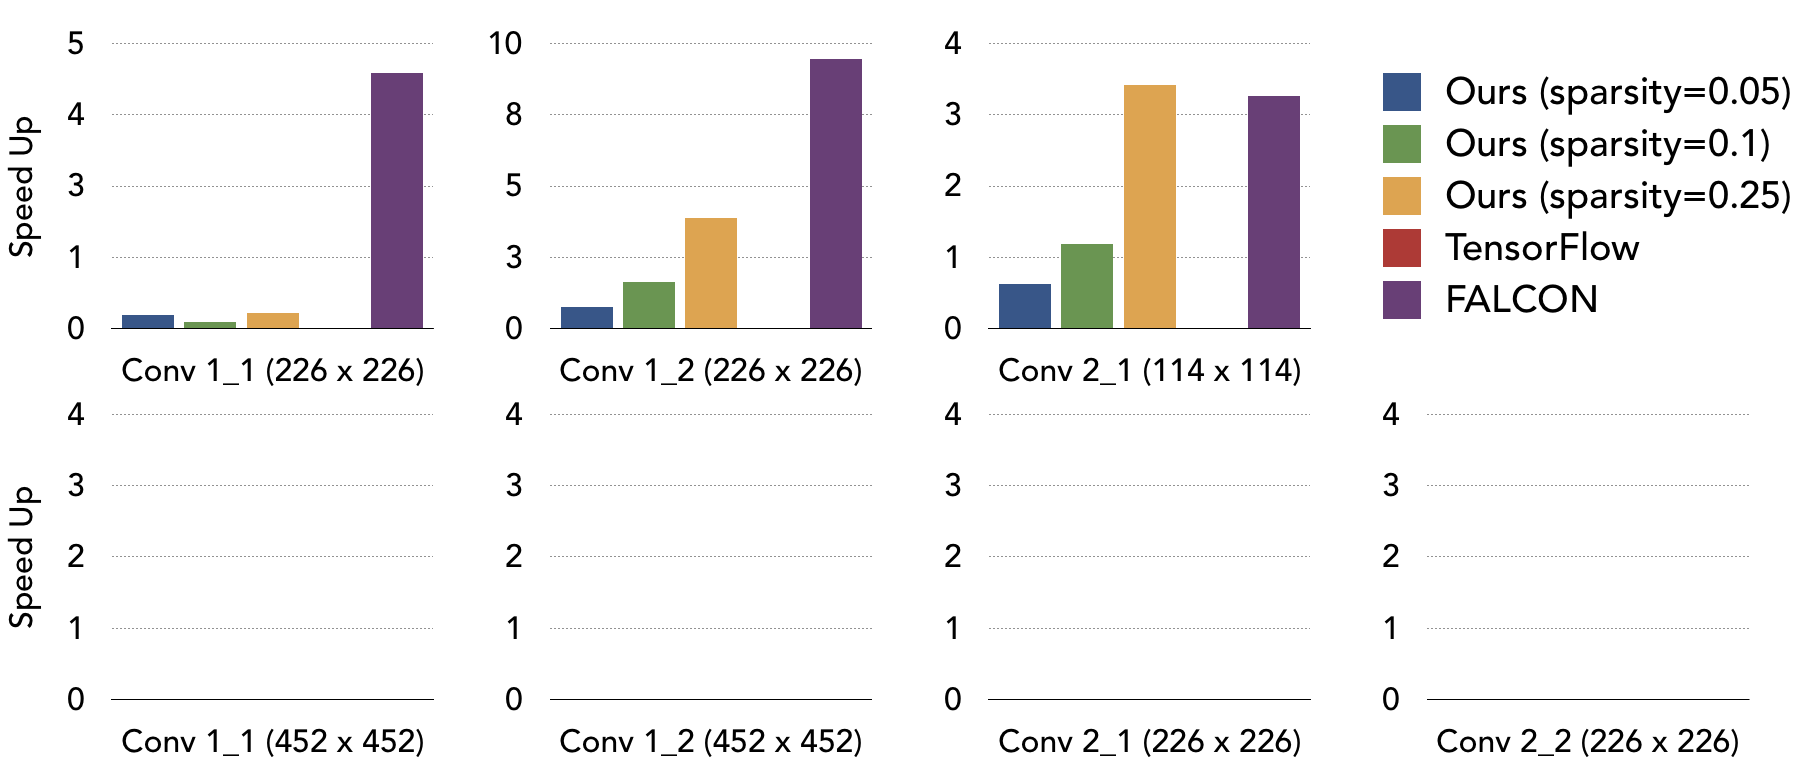
\includegraphics[width=\textwidth]{falcon_tf}
    \label{fig:falcon_tf}
\end{figure}

\begin{figure}[t]
	\centering
	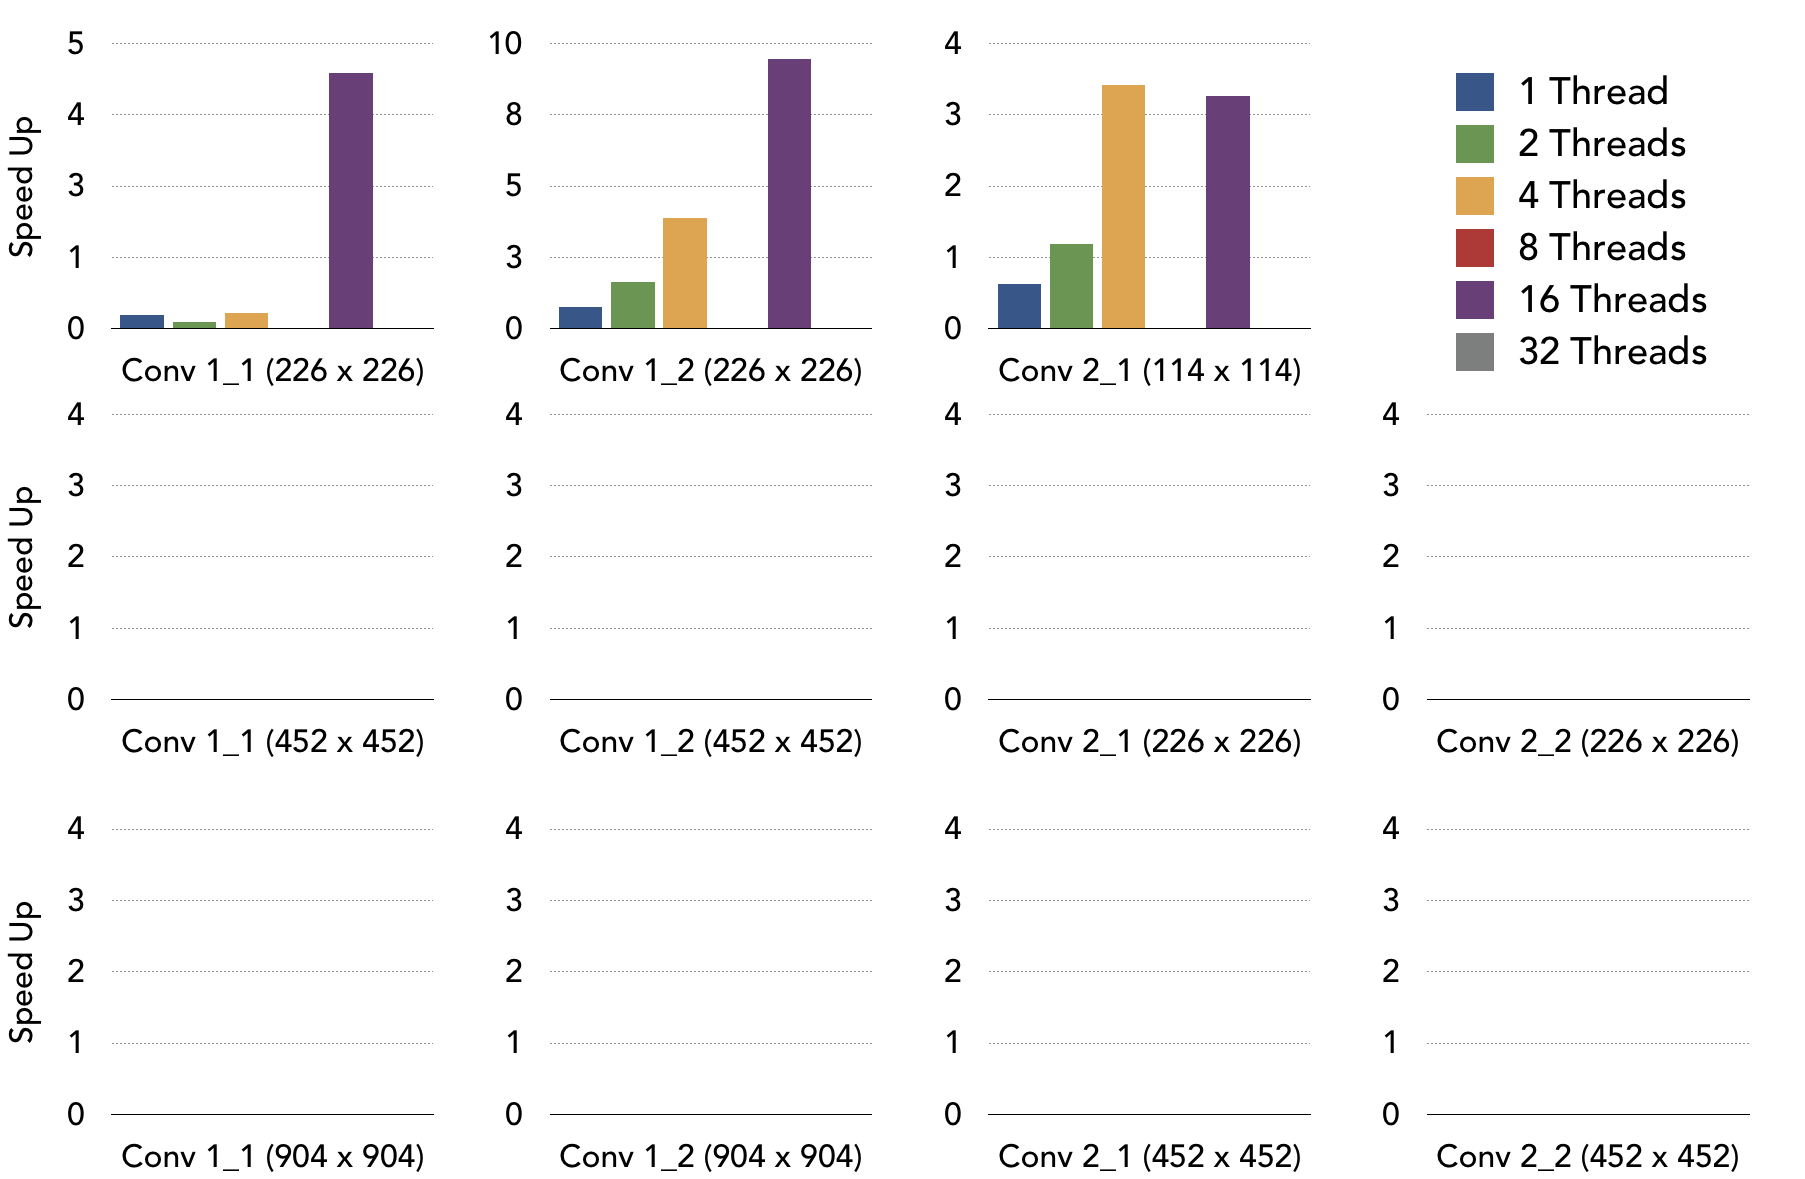
\includegraphics[width=\textwidth]{scaling}
    \label{fig:scaling}
\end{figure}
\label{sec:eval}

\section{Conclusions}
\label{sec:conclusion}

\bibliographystyle{abbrv}
\nocite{*}
{\bibliography{report}}

\end{document}
